%% Use Cases Template File
%% Created by Tom Desair (http://www.tomdesair.com)
%% Downloadable at: http://www.tomdesair.com/downloads/use-case-latex-template.zip
%% Date Modified: 03/04/2012
%
% This work may be distributed and/or modified under the
% conditions of the LaTeX Project Public License, either version 1.3
% of this license or (at your option) any later version.
% The latest version of this license is in
%   http://www.latex-project.org/lppl.txt
% and version 1.3 or later is part of all distributions of LaTeX
% version 2005/12/01 or later.

\documentclass[a4paper, 10pt, oneside]{article}

%include the usecases package
\usepackage{usecases}
\usepackage{graphicx}
\DeclareGraphicsExtensions{.pdf,.png,.jpg}
\usepackage[margin=1in]{geometry}

\begin{document}
\begin{titlepage}
    \vspace*{75pt} %leave out given verticle space in a document
    \begin{center}
        {\Huge Edith Visual Editor}\\ [1cm]    %make title huge and have .5cm space in between
		{\Large Graham Baker\\
Walker Bohannan\\
Steve Marx    \\
Vikram Nilakantan\\
Jessica Penick\\
Eli Spiegel \\
}
    \today %put the date that the data is compiled
\vspace*{75pt}

<<<<<<< HEAD

\end{center}
\noindent This document describes how a user of Edith, an educational software designed to teach young computer scientists the basics of programming, will be able to interact with the program by developing a story. The visual interface of Edith is designed to graphically represent bits of code and let the user manipulate physical objects instead of using text. Edith should effectively teach young programmers some of the building blocks of programming. The visual interface will support the user creating new methods, control structures, and conditional statements by dragging and dropping graphic representations of code together. The Visual Editor must interact directly with the Object and Story creators in order to implement the user's visual abstraction of code. When the user completes the story, the visual interface will be able to convert the shapes and symbols into JavaScript. This visual representation will give young coders instant gratification, encouraging them to progress to text-based programming. 

=======
\end{center}
\noindent This document describes how a user of Edith, an educational software designed to teach young computer scientists the basics of programming, will be able to interact with the program by developing a story. The visual interface of Edith is designed to graphically represent bits of code and let the user manipulate physical objects instead of using text. Edith should effectively teach young programmers some of the building blocks of programming. The visual interface will support the user creating new methods, control structures, and conditional statements by dragging and dropping graphic representations of code together. The Visual Editor must interact directly with the Object and Story creators in order to implement the user's visual abstraction of code. When the user completes the story, the visual interface will be able to convert the shapes and symbols into JavaScript. This visual representation will give young coders instant gratification, encouraging them to progress to text-based programming. 
	
>>>>>>> 730c584a87d58eaa99e755eaef9977bc9d9f8170
	\vspace*{\fill}
\end{titlepage}

%Sometimes it is a good idea to put domain objects in \texttt{}
%The template and the descriptions are based on the book Applying UML and Patterns: 
%An Introduction to Object-Oriented Analysis and Design and Iterative Development
%(3rd Edition) by Craig Larman.
\begin{usecase}

\addtitle{Introduction}{} 



%Main Success Scenario: A typical, unconditional happy path scenario of success.
\addscenario{}{
\item []\indent Edith is educational software designed to introduce new computer science students to programming.  New students of any age can learn basic object-oriented programming concepts prior to learning a particular programming language in detail (syntax, data types and structures, etc.).  Edith provides a graphical user interface through which users can create a "script" that animates a 2-D character, or sprite, provided by the program.  The user creates the script by piecing together provided blocks of program structure in a functional way.  Users may create games and share their creations with others. Similar programs (e.g., Alice) have been shown to increase the interest level and retention of students taking their first programming classes.    Edith will be written primarily in JavaScript and will be available over the internet.  After initial development, the software will be open-source to allow further development and additional educational opportunities.\newline	

<<<<<<< HEAD
\indent The Visual Editor (VE) module will provide a visual programming language editor (in essence, an integrated development environment(IDE)).  The VE will allow users to arrange programming elements to create an animation sequence; programming elements will include methods, variables, control statements, etc. The VE will, while enforcing syntax rules, convert the program into JavaScript, which will be used by other modules. The VE aims to create an interface that it is easy to use, and following its name, will create a view that is always immediately ready to be seen. Since it will be using JavaScript, there will be no wait for compiling to see if the code "works," on the view of the Programmer. Rather, the code, or sequence of events defined by the user, will be always ready to run unless a script notifies the user otherwise.\newline

\indent The VE will be able to directly interact with two other Edith modules, Object Creator and Story Creator, while still being able to run independently.  It will provide the Object Creator an interface for defining objects, and the Story Creator an interface for defining animations.  In short, the VE will be able to run its own display view and integrate into the views of other Edith modules. The VE will provide not only an interface for the Programmer to create his own code, but also for the other modules to implement code provided by the visual editor.\newline	
=======
\indent The Visual Editor (VE) module will provide a visual programming language editor (in essence, an integrated development environment(IDE)).  The VE will allow users to arrange programming elements to create an animation sequence; programming elements will include methods, variables, control statements, etc. The VE will, while enforcing syntax rules, convert the program into JavaScript, which will be used by other modules. The VE aims to create an interface that it is easy to use, and following its name, will create a view that is always immediately ready to be seen. Since it will be using JavaScript, there will be no wait for compiling to see if the code "works," on the view of the end-user. Rather, the code, or sequence of events defined by the user, will be always ready to run unless a script notifies the user otherwise.\newline

\indent The VE will be able to directly interact with two other Edith modules, Object Creator and Story Creator, while still being able to run independently.  It will provide the Object Creator an interface for defining objects, and the Story Creator an interface for defining animations.  In short, the VE will be able to run its own display view and integrate into the views of other Edith modules. The VE will provide not only an interface for the end-user to create his own code, but also for the other modules to implement code provided by the visual editor.\newline	
>>>>>>> 730c584a87d58eaa99e755eaef9977bc9d9f8170

\indent The user will be able to export his program in JavaScript/JavaScript Object Notation (JSON) format. JSON is an efficient data interchange text format that is language independent. The purpose of this is to again encourage learning of coding to our target users -- young students who wish to learn more about what they are doing as far as coding, what their changes look like from a lower level than the visual editing.\newline
}

\end{usecase}


\begin{usecase}

\addtitle{Use Case 1}{Edit variable} 

%Primary Actor: Calls on the system to deliver its services.
\addfield{Primary Actor:}{Programmer}

%Preconditions: What must be true on start and worth telling the reader?
\addfield{Preconditions:}{Method exists which has a variable parameter.}
%when multiple
%\additemizedfield{Preconditions:}{} 

%Postconditions: What must be true on successful completion and worth telling the reader
\addfield{Postconditions:}{Variable is assigned value given by user.}
%when multiple
%\additemizedfield{Preconditions:}{}

%Main Success Scenario: A typical, unconditional happy path scenario of success.
\addscenario{Main Success Scenario:}{
    \item[1.] User selects variable
    \item[2.] User changes the parameter 
    \item[3.] Check variable type to make sure it is compatible with method
    \item[4.] Variable is saved in method
}

%Extensions: Alternate scenarios of success or failure.
\addscenario{Extensions:}{
	\item[3.a] Invalid type data:
		\begin{enumerate}
		\item[1.]  Incorrect input.
		\item[1.a] Boundary warning.
		\item[1.b] Wrong type.
		\item[2.]  User returns to step 1 or exits.
		\end{enumerate}
	\item[3.b] Compatible type:
		\begin{enumerate}
		\item[1.] System accepts input and saves parameter.
		\end{enumerate}				
}

%Non-Functional Requirements Needed: Related Non-Functional Requirements Needed.
\addscenario{Non-Functional      Requirements Needed:}{
	\item Learning Experience.
	\item Usability.
}
%Miscellaneous: Such as open issues/questions
%\addfield{Open Issues:}{}
\end{usecase}

\begin{usecase}

\addtitle{Use Case 2}{Dragging and dropping functionality for methods} 

%Primary Actor: Calls on the system to deliver its services.
\addfield{Primary Actor:}{Programmer}



%Preconditions: What must be true on start and worth telling the reader?
\addfield{Preconditions:}{There is a method for which it is possible to be selected.}
%when multiple
%\additemizedfield{Preconditions:}{} 

%Postconditions: What must be true on successful completion and worth telling the reader
\addfield{Postconditions:}{Method is now ready to be used.}
%when multiple
%\additemizedfield{Preconditions:}{}

%Main Success Scenario: A typical, unconditional happy path scenario of success.
\addscenario{Main Success Scenario:}{
    \item[1.] User creates new variable and selects it.
    \item[2.] They can now drag and drop the variable in the boundaries provided.

}

%Extensions: Alternate scenarios of success or failure.
\addscenario{Extensions:}{
	\item[1.] Invalid drop location:
		\begin{enumerate}
		\item[1.a.] The user attempts to drag the variable outside of acceptable boundaries, the variable will now be "locked" inside of acceptable boundary.

		\end{enumerate}

}

%Non-Functional Requirements Needed: Related Non-Functional Requirements Needed.
\addscenario{Non-Functional Requirements Needed:}{
	\item Learning Experience.
	\item Usability.
}


%Miscellaneous: Such as open issues/questions
%\addfield{Open Issues:}{}

\end{usecase}

\begin{usecase}

\addtitle{Use Case 3}{Instantiating a conditional statement } 

%Primary Actor: Calls on the system to deliver its services.
\addfield{Primary Actor:}{Programmer}

%Postconditions: What must be true on successful completion and worth telling the reader
\addfield{Postconditions:}{A conditional is instantiated.}
%when multiple
%\additemizedfield{Preconditions:}{}

%Main Success Scenario: A typical, unconditional happy path scenario of success.
\addscenario{Main Success Scenario:}{
    \item[1.] A user drags and drops a conditional statement
    \item[2.] They change the parameter (e.g. if this) 
    \item[3.] The inside of the conditional is then dragged and dropped (e.g. then that).

}

%Non-Functional Requirements Needed: Related Non-Functional Requirements Needed.
\additemizedfield{Non-Functional Requirements Needed:}{
	\item Learning Experience.
	\item Usability.
}


%Miscellaneous: Such as open issues/questions
%\addfield{Open Issues:}{}

\end{usecase}

\begin{usecase}

\addtitle{Use Case 4}{Instantiating a Boolean Operator} 

%Primary Actor: Calls on the system to deliver its services.
\addfield{Primary Actor:}{Programmer}


%Postconditions: What must be true on successful completion and worth telling the reader
\addfield{Postconditions:}{A boolean operator is instantiated}
%when multiple
%\additemizedfield{Preconditions:}{}

%Main Success Scenario: A typical, unconditional happy path scenario of success.
\addscenario{Main Success Scenario:}{
    \item A user drags and drops an operation (e.g. and, or, not)
    \item the user sets the two variables or expressions
}



%Non-Functional Requirements Needed: Related Non-Functional Requirements Needed.
\addscenario{Non-Functional Requirements Needed:}{
	\item Learning Experience.
	\item Usability.
}


%Miscellaneous: Such as open issues/questions
%\addfield{Open Issues:}{}

\end{usecase}


\begin{usecase}

\addtitle{Use Case 5}{ Connecting actions} 

%Primary Actor: Calls on the system to deliver its services.
\addfield{Primary Actor:}{Programmer}



%Preconditions: What must be true on start and worth telling the reader?
\addfield{Preconditions:}{There are two or more actions on the development board. }
%when multiple
%\additemizedfield{Preconditions:}{} 

%Postconditions: What must be true on successful completion and worth telling the reader
\addfield{Postconditions:}{The methods are connected.}
%when multiple
%\additemizedfield{Preconditions:}{}

%Main Success Scenario: A typical, unconditional happy path scenario of success.
\addscenario{Main Success Scenario:}{
    \item The method is draged and droped by the user  above or below the action they want to connect to
    \item The user releases the method 
}



%Non-Functional Requirements Needed: Related Non-Functional Requirements Needed.
\additemizedfield{Non-Functional Requirements Needed:}{
	\item Learning Experience.
	\item Usability.
}


%Miscellaneous: Such as open issues/questions
%\addfield{Open Issues:}{}

\end{usecase}


\begin{usecase}

\addtitle{Use Case 6}{Delete a method} 

%Primary Actor: Calls on the system to deliver its services.
\addfield{Primary Actor:}{Programmer}



%Preconditions: What must be true on start and worth telling the reader?
\addfield{Preconditions:}{There are methods on the development board}
%when multiple
%\additemizedfield{Preconditions:}{} 

%Postconditions: What must be true on successful completion and worth telling the reader
\addfield{Postconditions:}{Selected methods are deleted}
%when multiple
%\additemizedfield{Preconditions:}{}

%Main Success Scenario: A typical, unconditional happy path scenario of success.
\addscenario{Main Success Scenario:}{
    \item The user selects a method or group of methods
    \item The user selects to delete the selected items
}

%Extensions: Alternate scenarios of success or failure.
\addscenario{Extensions:}{
	\item[2.a] Invalid type data:
		\begin{enumerate}
		\item[1.]  Incorrect input
		\item[2.] User returns to step 1 or exits
		\end{enumerate}

}

%Non-Functional Requirements Needed: Related Non-Functional Requirements Needed.
\additemizedfield{Non-Functional Requirements Needed:}{
	\item Learning Experience.
	\item Usability.
}


%Miscellaneous: Such as open issues/questions
%\addfield{Open Issues:}{}

\end{usecase}

\begin{usecase}

\addtitle{Use Case 7}{Delete a method} 

%Primary Actor: Calls on the system to deliver its services.
\addfield{Primary Actor:}{Programmer}



%Preconditions: What must be true on start and worth telling the reader?
\addfield{Preconditions:}{There are methods on the development board}
%when multiple
%\additemizedfield{Preconditions:}{} 

%Postconditions: What must be true on successful completion and worth telling the reader
\addfield{Postconditions:}{Selected methods are deleted}
%when multiple
%\additemizedfield{Preconditions:}{}

%Main Success Scenario: A typical, unconditional happy path scenario of success.
\addscenario{Main Success Scenario:}{
    \item The user selects a method or group of methods
    \item The user selects to delete the selected items
}

%Extensions: Alternate scenarios of success or failure.
\addscenario{Extensions:}{
    \item[2.a] Invalid type data:
		\begin{enumerate}
		\item[1.]  Incorrect input
		\item[2.] User returns to step 1 or exits
		\end{enumerate}

}

%Non-Functional Requirements Needed: Related Non-Functional Requirements Needed.
\additemizedfield{Non-Functional Requirements Needed:}{
	\item Learning Experience.
	\item Usability.
}


%Miscellaneous: Such as open issues/questions
%\addfield{Open Issues:}{}

\end{usecase}

\begin{usecase}

\addtitle{Use Case 8}{Instantiating a Loop} 

%Primary Actor: Calls on the system to deliver its services.
\addfield{Primary Actor:}{Programmer}



%Preconditions: What must be true on start and worth telling the reader?
\addfield{Preconditions:}{Add method which does have a variable parameter.}
%when multiple
%\additemizedfield{Preconditions:}{} 

%Postconditions: What must be true on successful completion and worth telling the reader
\addfield{Postconditions:}{A loop is instantiated}
%when multiple
%\additemizedfield{Preconditions:}{}

%Main Success Scenario: A typical, unconditional happy path scenario of success.
\addscenario{Main Success Scenario:}{
    \item The user drags and drop a loop to the development board
    \item The user then inputs the conditionals for the loop and its exit conditions. 
}

%Extensions: Alternate scenarios of success or failure.
\addscenario{Extensions:}{
	\item[2.a] Invalid input:
		\begin{enumerate}
		\item[1.]  User returns to step 1 or exits
    	\end{enumerate}

}

%Non-Functional Requirements Needed: Related Non-Functional Requirements Needed.
\additemizedfield{Non-Functional Requirements Needed:}{
	\item Learning Experience.
	\item Usability.
}


%Miscellaneous: Such as open issues/questions
%\addfield{Open Issues:}{}

\end{usecase}

\begin{usecase}

\addtitle{Use Case 9}{Creating a new Action} 

%Primary Actor: Calls on the system to deliver its services.
\addfield{Primary Actor:}{Programmer}



%Preconditions: What must be true on start and worth telling the reader?
\addfield{Preconditions:}{None.}
%when multiple
%\additemizedfield{Preconditions:}{} 

%Postconditions: What must be true on successful completion and worth telling the reader
\addfield{Postconditions:}{If first method, the box is made, if attaching to another method, the boxes are connected}
%when multiple
%\additemizedfield{Preconditions:}{}

%Main Success Scenario: A typical, unconditional happy path scenario of success.
\addscenario{Main Success Scenario:}{
    \item The user selects the new method button
    \item Drags the method into the workbox 
    \item then the method prompts the user to give arguments for that specific action 
    \item If arguments are compatible, the method is created

}

%Extensions: Alternate scenarios of success or failure.
\addscenario{Extensions:}{
	\item[2.a] Invalid input:
		\begin{enumerate}
		\item[1.]  User prompted to re-enter arguments
    	\end{enumerate}

}
\end{usecase}
\begin{usecase}

<<<<<<< HEAD
=======
\addtitle{Use Case 12}{Exporting Project} 

%Primary Actor: Calls on the system to deliver its services.
\addfield{Primary Actor:}{End-User}



%Preconditions: What must be true on start and worth telling the reader?
\addfield{Preconditions:}{Project contains atleast one method/action}
%when multiple
%\additemizedfield{Preconditions:}{} 

%Postconditions: What must be true on successful completion and worth telling the reader
\addfield{Postconditions:}{If successful, the user should get a message on how to share the file with another user.}
%when multiple
%\additemizedfield{Preconditions:}{}

%Main Success Scenario: A typical, unconditional happy path scenario of success.
\addscenario{Main Success Scenario:}{
    \item The user selects the Export button
    \item The system generates an export-ready file for the user
    \item The system gives the user options on how to share the file

}

%Extensions: Alternate scenarios of success or failure.
\addscenario{Extensions:}{
	\item[2.a] No methods existed.
		\begin{enumerate}
		\item[1.]  User prompted to add a method/action before trying to export again.
    	\end{enumerate}

}

%Non-Functional Requirements Needed: Related Non-Functional Requirements Needed.
\additemizedfield{Non-Functional Requirements Needed:}{
	\item Usability.
}


%Miscellaneous: Such as open issues/questions
%\addfield{Open Issues:}{}

\end{usecase}
% New Page for Use Case Diagram

\begin{usecase}

\addtitle{Use Case 13}{Importing Project} 

%Primary Actor: Calls on the system to deliver its services.
\addfield{Primary Actor:}{End-User}



%Preconditions: What must be true on start and worth telling the reader?
\addfield{Preconditions:}{User has a valid export file to import}
%when multiple
%\additemizedfield{Preconditions:}{} 

%Postconditions: What must be true on successful completion and worth telling the reader
\addfield{Postconditions:}{If successful, the visual editor should load the actions/methods present in the export file}
%when multiple
%\additemizedfield{Preconditions:}{}

%Main Success Scenario: A typical, unconditional happy path scenario of success.
\addscenario{Main Success Scenario:}{
    \item The user selects the Import button
    \item The system reads and loads in methods/actions from file
    \item Canvas/Display updates with GUI versions of the methods with appropriate parameters.
    \item The user is now available to edit/add methods or actions to the file

}

%Extensions: Alternate scenarios of success or failure.
\addscenario{Extensions:}{
	\item[1] Export file missing or corrupt
		\begin{enumerate}
		\item[1.a]  User prompted to re-upload a file with the correct file structure.
    	\end{enumerate}

}

%Non-Functional Requirements Needed: Related Non-Functional Requirements Needed.
\additemizedfield{Non-Functional Requirements Needed:}{
	\item Usability
	\item Learning Experience
}
>>>>>>> 730c584a87d58eaa99e755eaef9977bc9d9f8170


%Miscellaneous: Such as open issues/questions
%\addfield{Open Issues:}{}

\end{usecase}

\begin{usecase}

\addtitle{Use Case 10}{Add Sprite Object} 

%Primary Actor: Calls on the system to deliver its services.
\addfield{Primary Actor:}{Programmer}



%Preconditions: What must be true on start and worth telling the reader?
\addfield{Preconditions:}{None.}
%when multiple
%\additemizedfield{Preconditions:}{} 

%Postconditions: What must be true on successful completion and worth telling the reader
\addfield{Postconditions:}{New Sprite Object has been added to the visual editor and methods/actions can be added to it.}
%when multiple
%\additemizedfield{Preconditions:}{}

%Main Success Scenario: A typical, unconditional happy path scenario of success.
\addscenario{Main Success Scenario:}{
    \item The user selects the New Sprite button
    \item The user fills in basic details of the Sprite
    \item The editor updates with the ability to add new methods/actions to the Sprite.

}

%Extensions: Alternate scenarios of success or failure.
\addscenario{Extensions:}{
	\item[1] None.

}

%Non-Functional Requirements Needed: Related Non-Functional Requirements Needed.
\additemizedfield{Non-Functional Requirements Needed:}{
	\item Usability
	\item Learning Experience
}


%Miscellaneous: Such as open issues/questions
%\addfield{Open Issues:}{}

\end{usecase}

\begin {usecase}


\addtitle{Use Case 10}{Delete Sprite Object} 

%Primary Actor: Calls on the system to deliver its services.
\addfield{Primary Actor:}{Programmer}



%Preconditions: What must be true on start and worth telling the reader?
\addfield{Preconditions:}{The selected Sprite object exists}
%when multiple
%\additemizedfield{Preconditions:}{} 

%Postconditions: What must be true on successful completion and worth telling the reader
\addfield{Postconditions:}{Selected Sprite object has been removed from visual editor.}
%when multiple
%\additemizedfield{Preconditions:}{}

%Main Success Scenario: A typical, unconditional happy path scenario of success.
\addscenario{Main Success Scenario:}{
    \item The user selects a Sprite from the visual editor.
    \item The user clicks on the Remove Sprite button
    \item System throws a confirmation box to make sure removal was triggered on purpose
    \item The sprite and its associated methods/actions are removed from the visual editor

}

%Extensions: Alternate scenarios of success or failure.
\addscenario{Extensions:}{
	\item[1] User selects 'Remove Sprite' when none exists
	\item[1.a.] System tells user that a Sprite must be first created to remove it.

}

%Non-Functional Requirements Needed: Related Non-Functional Requirements Needed.
\additemizedfield{Non-Functional Requirements Needed:}{
	\item Usability
	\item Learning Experience
}


%Miscellaneous: Such as open issues/questions
%\addfield{Open Issues:}{}

\end{usecase}

% New Page for Use Case Diagram
\newpage

\begin{usecase}
\addtitle{Use Case Diagram}{}
% Use case diagram inserted
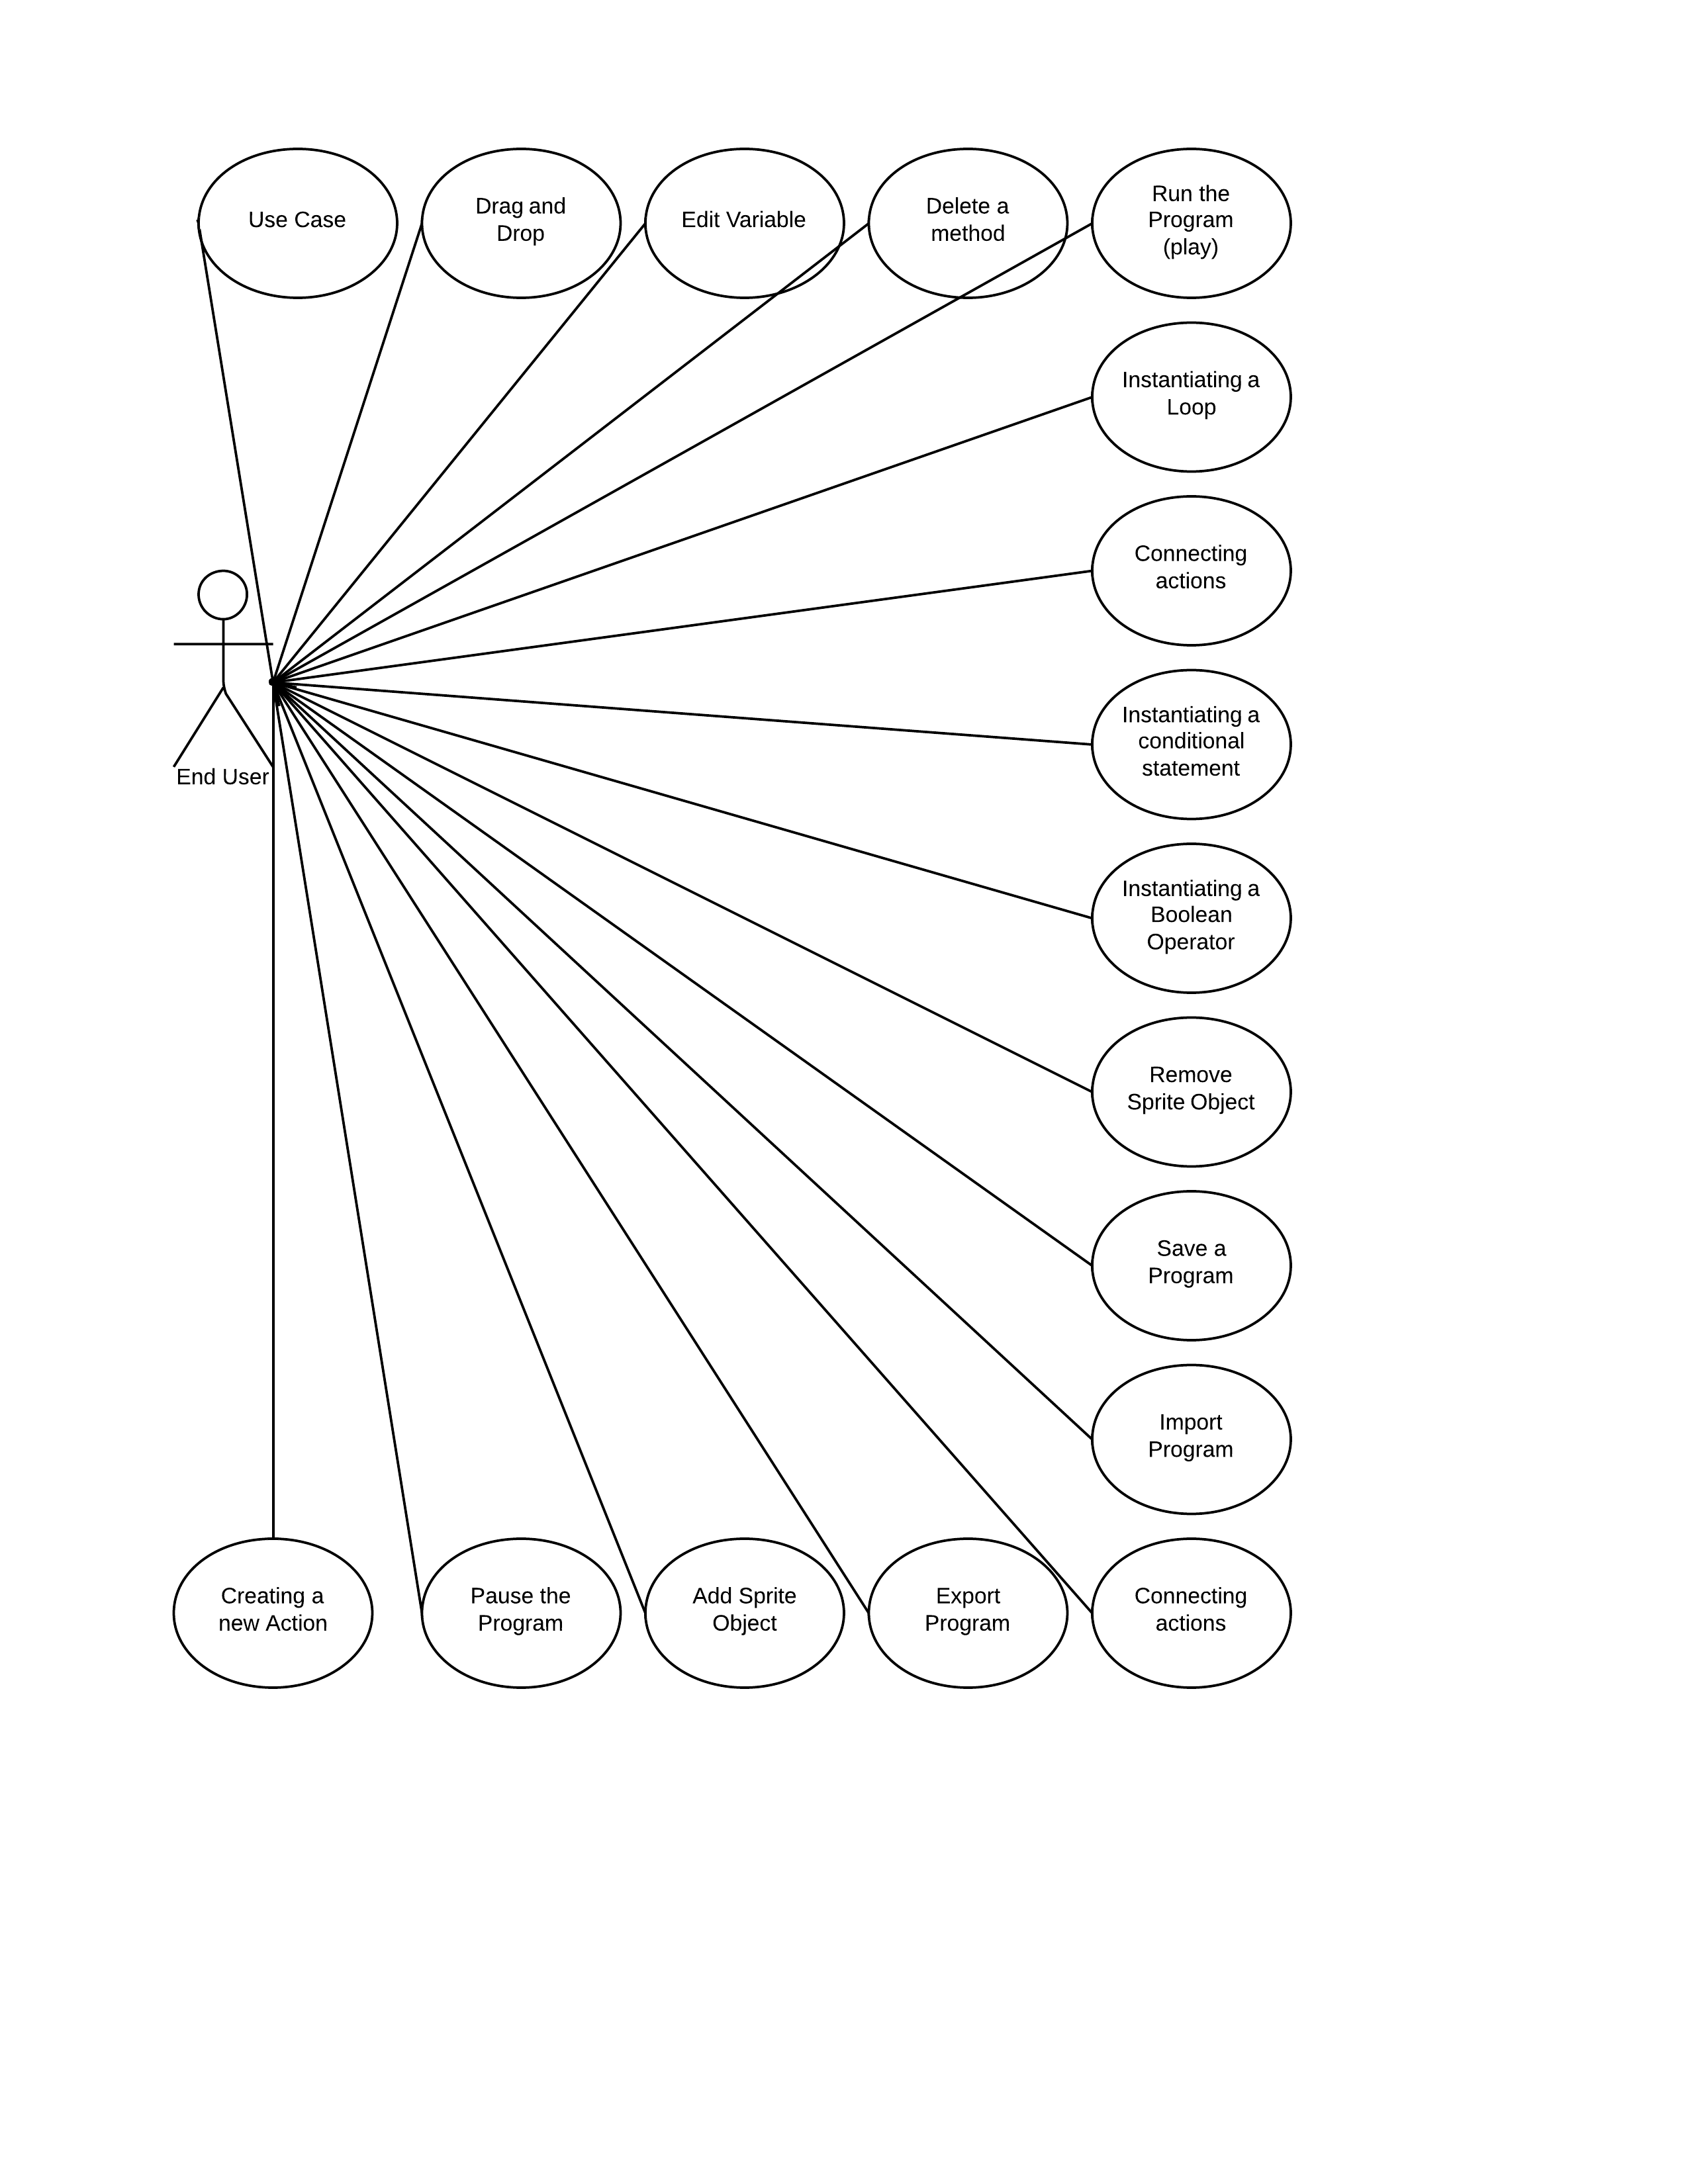
\includegraphics[scale=.36]{req_uml_diag.png}
\end{usecase}


\begin{usecase}

\addtitle{Non-Functional Requirements}{} 



%Main Success Scenario: A typical, unconditional happy path scenario of success.
\addscenario{Usability}{
 \item []Training should not be required for users to effectively use the module.  
Module documentation and basic age-specific computer knowledge should provide sufficient guidance.
The module should allow the user to recover from errors with informative and understandable error messages. 
}

\addscenario{Documentation}{
\item []The module will provide documentation that allows users to easily begin using the system.
  
}
\addscenario{Modifiability}{
 \item [] The module will have the flexibility to allow feature expansion over time.
}
\addscenario{Privacy}{
\item [] The user's work will remain private/secure unless the user chooses to share it. 
}
\addscenario{Student Learning Experience}{
 \item [] In order to support the learning of young computing students, the module will provide
an engaging interest that increases their interest in the subject.  Effectiveness may be measured by student retention rates and self-reported interest levels.  
}
\addscenario{Platform}{
\item []  Users will be able to run the module from Windows or Mac
}
\addscenario{Open Source}{
 \item []After initial development, the source code will be open and redistributed with improvements by anyone.
}

\end{usecase}

\begin{usecase}

\addtitle{Glossary and References}{} 

\addscenario{Glossary}{

\item[Sprite -- ]	A term borrowed from another visual programming editor "Scratch" (found here: http://scratch.mit.edu/). A sprite is like an instantiation of a class in that it is a character with actions (methods) that the programmer might define via the drag and drop IDE.\newline
<<<<<<< HEAD

\item[Development Board -- ]	Or the "working area." This is the area of the IDE that the programmer drags the graphic representations of code to in order to develop programs. Not to be confused with the canvas where the actions specified by the code take place (much like the console of a more typical IDE).\newline
}
\addscenario{References}{
\item [ALICE -- ]	ALICE is a 3D visual programming editor which allows student to drag and drop pieces to create a program. The program, as well as more information on the nature of the program, can be found at alice.org.\newline

\item[LaTeX Template -- ]	This use cases template was created by Tom Desair and can be downloaded at http://www.tomdesair.com/downloads/use-case-latex-template.zip

=======

\item[Development Board -- ]	Or the "working area." This is the area of the IDE that the programmer drags the graphic representations of code to in order to develop programs. Not to be confused with the canvas where the actions specified by the code take place (much like the console of a more typical IDE).\newline
}
\addscenario{References}{
\item [ALICE -- ]	ALICE is a 3D visual programming editor which allows student to drag and drop pieces to create a program. The program, as well as more information on the nature of the program, can be found at alice.org.\newline

\item[LaTeX Template -- ]	This use cases template was created by Tom Desair and can be downloaded at http://www.tomdesair.com/downloads/use-case-latex-template.zip

>>>>>>> 730c584a87d58eaa99e755eaef9977bc9d9f8170
}

\end{usecase}


\end{document}
